%##################################################################################################

\documentclass[11pt,letterpaper]{report}
%##################################################################################################

\usepackage{color}
    \definecolor{dark_blue}{rgb}{0,0,0.6}
    \definecolor{light_blue}{rgb}{0,0.4,0.8}
    \definecolor{dark_vilet}{rgb}{0.4,0,0.4}
\usepackage{fancybox}
\usepackage{wallpaper}
\usepackage{url}
\usepackage[colorlinks,
            linkcolor=dark_vilet,
            citecolor=light_blue,
            urlcolor=dark_blue]{hyperref}
\usepackage{colortbl}
\usepackage{amssymb}
\usepackage{amsmath}
\usepackage{graphicx}
\usepackage{algorithm}
\usepackage{algorithmic}
%\usepackage[square,comma,sort&compress]{natbib}
\usepackage[Sonny]{fncychap}
\usepackage{fancyhdr}
\usepackage[margin=1.5in]{geometry}
\usepackage{titletoc}
\usepackage[scaled=.92]{helvet}
\usepackage{mathptmx}
\usepackage{subfigure}
\usepackage{xspace}
\usepackage{multirow}
\usepackage[raggedright]{sidecap}

\renewcommand{\headrulewidth}{0.5pt}
\renewcommand{\footrulewidth}{0.5pt}
\ChTitleVar{\huge\sf}
\ChNameVar{\Huge\sf}
\rhead{}

\newcommand{\cdl}[1]{\textsf{#1}}
\newenvironment{link_url}
{\begin{description}
    \item}
{\end{description}}
\newenvironment{cmd_line}
{\begin{description}
    \item}
{\end{description}}

\newcommand{\ignore}[1]{}
\newcommand{\tabwidth}[0]{.45\linewidth}
\newcommand{\figwidth}[0]{.48\linewidth}

\newcommand\prjfnt{{\small \fontfamily{pag}\selectfont{}}\xspace}
\newcommand\gefnt{{\small \fontfamily{ppl}\selectfont{}}\xspace}
\newcommand{\PLASMA}{{\prjfnt{PLASMA}}\xspace}
\newcommand{\MAGMA}{{\prjfnt{MAGMA}}\xspace}
\newcommand{\TBLAS}{{\prjfnt{TBLAS}}\xspace}
\newcommand{\PBLAS}{{\prjfnt{PBLAS}}\xspace}
\newcommand{\PESSL}{{\prjfnt{PESSL}}\xspace}
\newcommand{\ESSL}{{\prjfnt{ESSL}}\xspace}
\newcommand{\SMPSS}{{\prjfnt{SMPSs}}\xspace}
\newcommand{\SMPSs}{{\prjfnt{SMPSs}}\xspace}
\newcommand{\MKL}{{\prjfnt{MKL}}\xspace}
\newcommand{\SCALAPACK}{{\prjfnt{ScaLAPACK}}\xspace}
\newcommand{\LAPACK}{{\prjfnt{LAPACK}}\xspace}
\newcommand{\LINPACK}{{\prjfnt{LINPACK}}\xspace}
\newcommand{\EISPACK}{{\prjfnt{EISPACK}}\xspace}
\newcommand{\DPOTRF}{{\gefnt{DPOTRF}}\xspace}
\newcommand{\DGEQRF}{{\gefnt{DGEQRF}}\xspace}
\newcommand{\DGETRF}{{\gefnt{DGETRF}}\xspace}
\newcommand{\DGEMM}{{\gefnt{DGEMM}}\xspace}
\newcommand{\BLAS}{{\gefnt{BLAS}}\xspace}
\newcommand{\BLACS}{{\gefnt{BLACS}}\xspace}
\newcommand{\dgemm}{{\gefnt{dgemm-seq}}\xspace}
\newcommand{\dssrfb}{{\gefnt{dssrfb-seq}}\xspace}
\newcommand{\dssssm}{{\gefnt{dssssm-seq}}\xspace}
\newcommand{\Intel}{{\gefnt{Intel64}}\xspace}
\newcommand{\Power}{{\gefnt{Power6}}\xspace}

%##################################################################################################

\begin{document}

%//////////////////////////////////////////////////////////////////////////////////////////////////

\thispagestyle{empty}
\begin{flushright}
\sf
\noindent
{\Huge\textbf{PLASMA Users' Guide}}
\rule[-1ex]{\textwidth}{5pt}\\[2.5ex]
{\Large\textbf{Parallel Linear Algebra Software for Multicore Architectures}} \\
\vspace{0.1in}
{\Large{Version 2.3}} \\
\vspace{0.1in}
{September 4th, 2010} \\
\vspace{0.1in}
{LAPACK Working Note XXX} \\
\vspace{0.1in}
{Technical Report UT-CS-XX-XXX} \\
\vspace{0.5in}

\noindent
Electrical Engineering and Computer Science \\
\textbf{University of Tennessee}
\vspace{0.2in}

\noindent
Mathematical \& Statistical Sciences \\
\textbf{University of Colorado Denver}
\vspace{0.2in}

\noindent
Electrical Engineering and Computer Science \\
\textbf{University of California at Berkeley}
\vspace{1.3in}

\noindent
\textcolor{white}{alphabetically}
\textcolor{white}{PIs:}
Jack Dongarra \\
Jakub Kurzak \\
Julien Langou \\

\textcolor{white}{core developers:}
Julie Langou \\
Hatem Ltaief \\
Piotr Luszczek \\
Asim YarKhan \\

\textcolor{white}{newcomers and students:}
Wesley Alvaro \\
Mathieu Faverge \\
Azzam Haidar \\
Joshua Hoffman \\

\textcolor{white}{past developers:}
Emmanuel Agullo \\
Alfredo Buttari \\
Bilel Hadri \\

\end{flushright}

%//////////////////////////////////////////////////////////////////////////////////////////////////

\tableofcontents
\pagenumbering{roman}
\pagestyle{fancy}
\setlength\parindent{0in}
\setlength\parskip{0.1in}
\sloppy
\rm

%//////////////////////////////////////////////////////////////////////////////////////////////////

%###################################################################################################

\chapter*{Preface}

PLASMA version 1.0 was released in November 2008 as a prototype software providing
\mbox{\em proof-of-concept} implementation of a linear equations solver based on LU factorization,
SPD linear equations solver based on Cholesky factorization and least squares problem solver based
on QR and LQ factorizations, with support for real arithmetic in double precision only.
The publication of this Users' Guide coincides with the September 2010 release of version 2.3 of
PLASMA, with the following set of features:

\begin{description}
\item[Linear Equation Solvers:]
Fast routines for solving dense systems of linear equations, symmetric positive systems
of linear equations and least square problems using a class of {\em tile algorithms} for
LU, Cholesky, QR and LQ factorizations.

\item[\mbox{Mixed-Precision} Solvers:]
\mbox{Mixed-precision} routines exploiting the speed advantage of single precision
by factorizing the matrix in single precision and using iterative refinement to achieve
``full'' double precision accuracy.

\item[Tall and Skinny Factorization Routines:]
Fast QR adn LQ factorization routines, closely related to a class of algorithms known as
{\em communication avoiding}, for factorizing matrices of heavily rectangular shape,
commonly referred to as {\em tall and skinny} matrices.

\item[Q Matrix Generation and Application Routines:]
Routines for implicit multiplication by the Q matrix resulting from the QR or LQ factorization
(application of the Householder reflectors) and routines for explicit generation of the Q
matrix (application of the Householder reflectors to an identity matrix).

\item[Matrix Inversion Routines:]
Fast routines for explicitly generating an \mbox{in-place} inverse of a matrix by
pipelining different stages of the computation using a dynamic scheduler with the
capability of data renaming for elimination of \mbox{anti-dependencies}.

\item[Tile Level 3 BLAS Routines:]
All Level 3 BLAS routines for matrices stored by tiles, the native storage format of PLASMA.

\item[Layout Translation Routines:]
Routines for efficient parallel \mbox{out-of-place} translation between the cannonical
\mbox{column-major} layout and the native PLASMA tile layout, as well as routines for
parallel and \mbox{cache-efficient} \mbox{in-place} translation (although more constrained
than the former one).

\item[Multiple Precision Support:]
Support for real arithmetic and complex arithmetic in single precision and double precision
(Z, D, C, S). Also, support for \mbox{mixed-precision} routines in real arithmetic and complex
arithmetic (ZC, DS).

\item[Flexible Interfaces:]
Three different interfaces with different levels of complexity and user's controll over the
operations: {\em basic interface} accepting matrices in cannonical \mbox{column-major} layout,
{\em tile interface} accepting matrices in tile layout and {\em tile asynchronous interface}
accepting matrices in tile layout and providing \mbox{non-blocking} computational calls.

\item[Workspace Allocation Routines:]
Convenient set of routines to handle workspace allocation where necessary, e.g., for passing
auxiliary data from the factorization routine to the solve routine.
Internal workspace allocation wherever possible.

\item[Rigorous Error Handling:]
Error codes closely following those returned by LAPACK for both illegal values of input
parameters and numerical defficiencies of the input matrices.

\item[Testing Suite:]
A set of tests derived from the LAPACK testing suite to exhaustively test the numerical routines
under normal conditions, as well as in the presence of illegal arguments and numerically deficient
matrices. Also a separate set of fast ``sanity'' tests.

\item[Timing Suite:]
A simple set of timing codes for measuring the performance of the basic interface and the tile
interface.

\item[Usage Examples:]
A set of usage examples for all routines in all precisions, ideal for quick cutting and pasting
into user's code.

\item[Extensive Documentation:]
Extensive documentation in the form of PDF manuals (Users' Guide, Reference Manual, TAU Guide,
Contributors' Guide), condensed ASCII and HTML files (README, LICENSE, Release Notes), an online
API Routine Reference and an online source code browser.

\item[Installer:]
Convenient Python installer for installation of PLASMA and all its software dependencies,
including: BLAS, CBLAS, LAPACK and LAPACK C Wrapper.
\end{description}

The current PLASMA release also implements many important software engineering practices,
including:

\begin{itemize}
    \item Thread safety,
    \item Support for Make and CMake build systems,
    \item Extensive comments in the source code using the Doxygen system,
    \item Support for multiple Unix OSes, as well as Microsoft Windows through a thin
          OS interaction layer,
    \item Clear software stack built from standard components, such as BLAS, CBLAS,
          LAPACK and LAPACK C Wrapper.
\end{itemize}

%###################################################################################################

%##################################################################################################

\chapter{Essentials}
\setcounter{page}{1}
\pagenumbering{arabic}

\section{PLASMA}

PLASMA is a software library, currently implemented using the FORTRAN and C programming languages,
and providing interfaces for FORTRAN and C.
It has been designed to be efficient on {\em homogeneous} multicore processors and \mbox{multi-socket}
systems of multicore processors. The name PLASMA is an acronym for {\em Parallel Linear Algebra
Software for Multi-core Architectures}.

PLASMA project website is located at:
\begin{link_url}
\url{http://icl.cs.utk.edu/plasma}
\end{link_url}

PLASMA software can be downloaded from:
\begin{link_url}
\url{http://icl.cs.utk.edu/plasma/software/}
\end{link_url}

PLASMA users' forum is located at:
\begin{link_url}
\url{http://icl.cs.utk.edu/plasma/forum/}
\end{link_url}
and can be used to post general questions and comments as well as to report technical problems.

%///////////////////////////////////////////////////////////////////////////////////////////////////

\section{Problems that PLASMA Can Solve}

PLASMA can solve dense systems of linear equations and linear least squares problems and associated
computations such as matrix factorizations.
Unlike LAPACK, currently PLASMA does not solve eigenvalue or singular value problems and does not
support band matrices.
Similarly to LAPACK, PLASMA does not support general sparse matrices.
For all supported types of computation the same functionality is provided for real and complex
matrices in single precision and double precision.

%///////////////////////////////////////////////////////////////////////////////////////////////////

\section{Computers for which PLASMA is Suitable}

PLASMA is designed to give high efficiency on homogeneous multicore processors and \mbox{multi-socket}
systems of multicore processors. As of today, the majority of such systems are \mbox{on-chip} symmetric
multiprocessors with classic \mbox{\em super-scalar} processors as their building blocks (x86 and alike)
augmented with \mbox{short-vector} SIMD extensions (SSE and alike).
A parallel software project MAGMA (Matrix Algebra on GPU and Multicore
Architectures), is being developed to address the needs of
heterogeneous (hybrid) systems, equipped with hardware accelerators,
such as GPUs.
\begin{link_url}
\url{http://icl.cs.utk.edu/magma}
\end{link_url}
The name MAGMA is an acronym for

%///////////////////////////////////////////////////////////////////////////////////////////////////

\section{PLASMA versus LAPACK and ScaLAPACK}

PLASMA has been designed to supercede LAPACK (and eventually ScaLAPACK), principally by restructuring the software
to achieve much greater efficiency, where possible, on modern computers based on multicore processors.
PLASMA also relies on new or improved algorithms.

Currently, PLASMA does not serve as a complete replacement of LAPACK due to limited functionality.
Specifically, PLASMA does not support band matrices and does not solve eigenvalue and singular
value problems.
At this point, PLASMA does not replace ScaLAPACK as software for distributed memory computers, since it
only supports \mbox{shared-memory} machines.

%///////////////////////////////////////////////////////////////////////////////////////////////////

\section{Error handling}

At the highest level (LAPACK interfaces), PLASMA reports errors through the
INFO integer parameter in the same manner as the LAPACK subroutines. 
INFO$<0$ means that there is an invalid argument in the calling sequence and no
computation has been performed; INFO$=0$ means that the computation has been
performed and no error has been issued; while INFO$>0$ means that a numerical
error has occured (e.g., no convergence in an eigensolver) or the input data is
(numerically) invalid (e.g., in xPOSV, the input matrix is not positive
definite). In any event, PLASMA returns the same INFO parameter as LAPACK.
When a numerical error is detected (INFO$>0$), the computation aborts as soon
as possible which implies that, in this case,
two different executions may very well have the current data in various states.
While the output state of LAPACK is predictible and
reproducible in the occurence of a numerical error, the one of PLASMA is not.

%///////////////////////////////////////////////////////////////////////////////////////////////////

\section{PLASMA and the BLAS}

LAPACK routines are written so that as much as possible of the computation is performed by calls
to the Basic Linear Algebra Subroutines (BLAS).
Highly efficient \mbox{machine-specific} implementations of the BLAS are available for most modern
processors, including \mbox{multi-threaded} implementations.

The parallel algorithms in PLASMA are built using a small set of sequential routines as building
blocks.
These routines are referred to as {\em core BLAS}.
Ideally, these routines would be implemented through monolithic \mbox{machine-specific} code, utilizing
to the maximum \mbox{a single} processing core (through the use of \mbox{short-vector} SIMD extensions
and appropriate cache and register blocking).

However, such \mbox{machine-specific} implementations are extremely
labor-intensive and covering the entire spectrum of available
architectures is not feasible.
Instead, the core BLAS routines are built in a somewhat suboptimal fashion, by using the
``standard'' BLAS routines as building blocks.
For that reason, just like LAPACK, PLASMA requires a highly optimized implementation of the BLAS
in order to deliver good performance.

Although the BLAS are not part of either PLASMA or LAPACK, FORTRAN code for the
BLAS is distributed with LAPACK, or can be obtained separately from Netlib:
\begin{link_url}
\url{http://www.netlib.org/blas/blas.tgz}
\end{link_url}
However, it has to be emphasized that this code is only the ``reference implementation'' (the definition
of the BLAS) and cannot be expected to deliver good performance. On most of today's machines it will
deliver performance an order of magnitude lower than that of optimized BLAS.

For information on available optimized BLAS libraries, as well as other \mbox{BLAS-related} questions,
please refer to the BLAS FAQ:
\begin{link_url}
\url{http://www.netlib.org/blas/faq.html}
\end{link_url}

%///////////////////////////////////////////////////////////////////////////////////////////////////

\section{Availability of PLASMA}

PLASMA is distributed in source code and is, for the most part, meant to be compiled from source
on the host system.
In certain cases, a \mbox{pre-built} binary may be provided along with the source code.
Such packages, built by the PLASMA developers, will be provided as separate archives on the
PLASMA download page:
\begin{link_url}
\url{http://icl.cs.utk.edu/plasma/software/}
\end{link_url}
The PLASMA team does not reserve exclusive right to provide such packages. They can be provided
by other individuals or institutions.
However, in case of problems with binary distributions acquired from other places, the provider
needs to be asked for support rather than PLASMA developers.

%///////////////////////////////////////////////////////////////////////////////////////////////////

\section{Commercial Use of PLASMA}

PLASMA is a freely available software package.
Thus it can be included in commercial packages.
The PLASMA team asks only that proper credit be given by citing this users' guide as the official
reference for PLASMA.

Like all software, this package is copyrighted. It is not trademarked.
However, if modifications are made that affect the interface,
functionality, or accuracy of the resulting software, the name of the
routine should be changed and the modifications to the software should
be noted in the modifier's documentation.

The PLASMA team will gladly answer questions regarding this software.
If modifications are made to the software, however, it is the responsibility of the individual or
institution who modified the routine to provide support.

%///////////////////////////////////////////////////////////////////////////////////////////////////

\section{Installation of PLASMA}

A PLASMA installer is available at:
\begin{link_url}
\url{http://icl.cs.utk.edu/plasma/software/}
\end{link_url}
Further details are provided in the  chapter \ref{install} \texttt{Installing PLASMA}.

%///////////////////////////////////////////////////////////////////////////////////////////////////

\section{Documentation of PLASMA}

PLASMA package comes with a variety of pdf and html documentation.
\begin{itemize}
	\item The PLASMA Users Guide (this document)
	\item The PLASMA README
	\item The PLASMA Installation Guide
	\item The PLASMA Routine Description
	\item The PLASMA and Tau Guide
	\item The PLASMA Routine browsing
\end{itemize}
You will find all of these in the documentation section on the PLASMA website \url{http://icl.cs.utk.edu/plasma}.


%///////////////////////////////////////////////////////////////////////////////////////////////////

\section{Support for PLASMA}

PLASMA has been thoroughly tested before release, using multiple
combinations of machine architectures, compilers and BLAS libraries.
The PLASMA project supports the package in the sense that reports of errors or poor performance
will gain immediate attention from the developers. Such reports -- and also descriptions of interesting
applications and other comments -- should be posted to the PLASMA users' forum:
\begin{link_url}
\url{http://icl.cs.utk.edu/plasma/forum/}
\end{link_url}

%///////////////////////////////////////////////////////////////////////////////////////////////////

\section{Funding}

The PLASMA project is funded in part by the National Science Foundation, U.~S. Department of Energy,
Microsoft Corporation, and The MathWorks Inc.

%###################################################################################################

%##################################################################################################

\chapter{Fundamentals}

%//////////////////////////////////////////////////////////////////////////////////////////////////

\section{Design Principles}

The main motivation behind the PLASMA project are performance shortcomings of \mbox{LAPACK}
and ScaLAPACK on shared memory systems, specifically systems consisting of multiple sockets
of multicore processors.
The three crucial elements that allow PLASMA to achieve performance greatly exceeding
that of LAPACK and ScaLAPACK are: the implementation of {\em tile algorithms}, the application
of {\em tile data layout} and the use of {\em dynamic scheduling}.
Although some performance benefits can be delivered by each one of these techniques
on its own, it is only the combination of all of them that delivers maximum performance
and highest hardware utilization.

%//////////////////////////////////////////////////////////

\subsection{Tile Algorithms}

Tile algorithms are based on the idea of processing the matrix by square tiles of relatively
small size, such that a tile fits entirely in one of the cache levels associated with one
core.
This way a tile can be loaded to the cache and processed completely before being evicted back
to the main memory.
Of the three types of cache misses, {\em compulsory}, {\em capacity} and {\em conflict},
the use of tile algorithms minimizes the number of capacity misses, since each operation
loads the amount of data that does not ``overflow'' the cache.

For some operations such as matrix multiplication and Cholesky factorization, translating
the classic algorithm to the tile algorithm is trivial.
In the case of matrix multiplication, the tile algorithm is simply a product of applying the
technique of {\em loop tiling} to the canonical definition of three nested loops.
It is very similar for the Cholesky factorization.
The \mbox{left-looking} definition of Cholesky factorization from LAPACK is a loop with
a sequence of calls to four routines: xSYRK (symmetric \mbox{rank-k} update), xPOTRF
(Cholesky factorization of a small block on the diagonal), xGEMM (matrix multiplication) and
xTRSM (triangular solve).
If the xSYRK, xGEMM and xTRSM operations are expressed with the canonical definition of three
nested loops and the technique of loop tiling is applied, the tile algorithm results.
Since the algorithm is produced by simple reordering of operations, neither the number of
operations nor numerical stability of the algorithm are affected.

The situation becomes slightly more complicated for LU and QR factorizations, where the
classic algorithms factorize an entire panel of the matrix (a block of columns) at every
step of the algorithm.
One can observe, however, that the process of matrix factorization is synonymous with introducing
zeros in approproate places and a tile algoritm can be fought of as one that zeroes one tile of
the matrix at a time.
This process is referred to as updating of a factorization or {\em incremental factorization}.
The process is equivalent to factorizing the top tile of a panel, then placing the upper
triangle of the result on top of the tile blow and factorizing again, then moving to the
next tile and so on.
Here, the tile LU and QR algorithms perform slightly more floating point operations and
require slightly more memory for auxiliary data.
Also, the tile LU factorization applies a different pivoting pattern and, as a result,
is less numerically stable than classic LU with full pivoting.
Numerical stability is not an issue in case of the tile QR, which relies on orthogonal
transformations (Householder reflections), which are numerically stable.

\begin{figure}[h!]
\centering
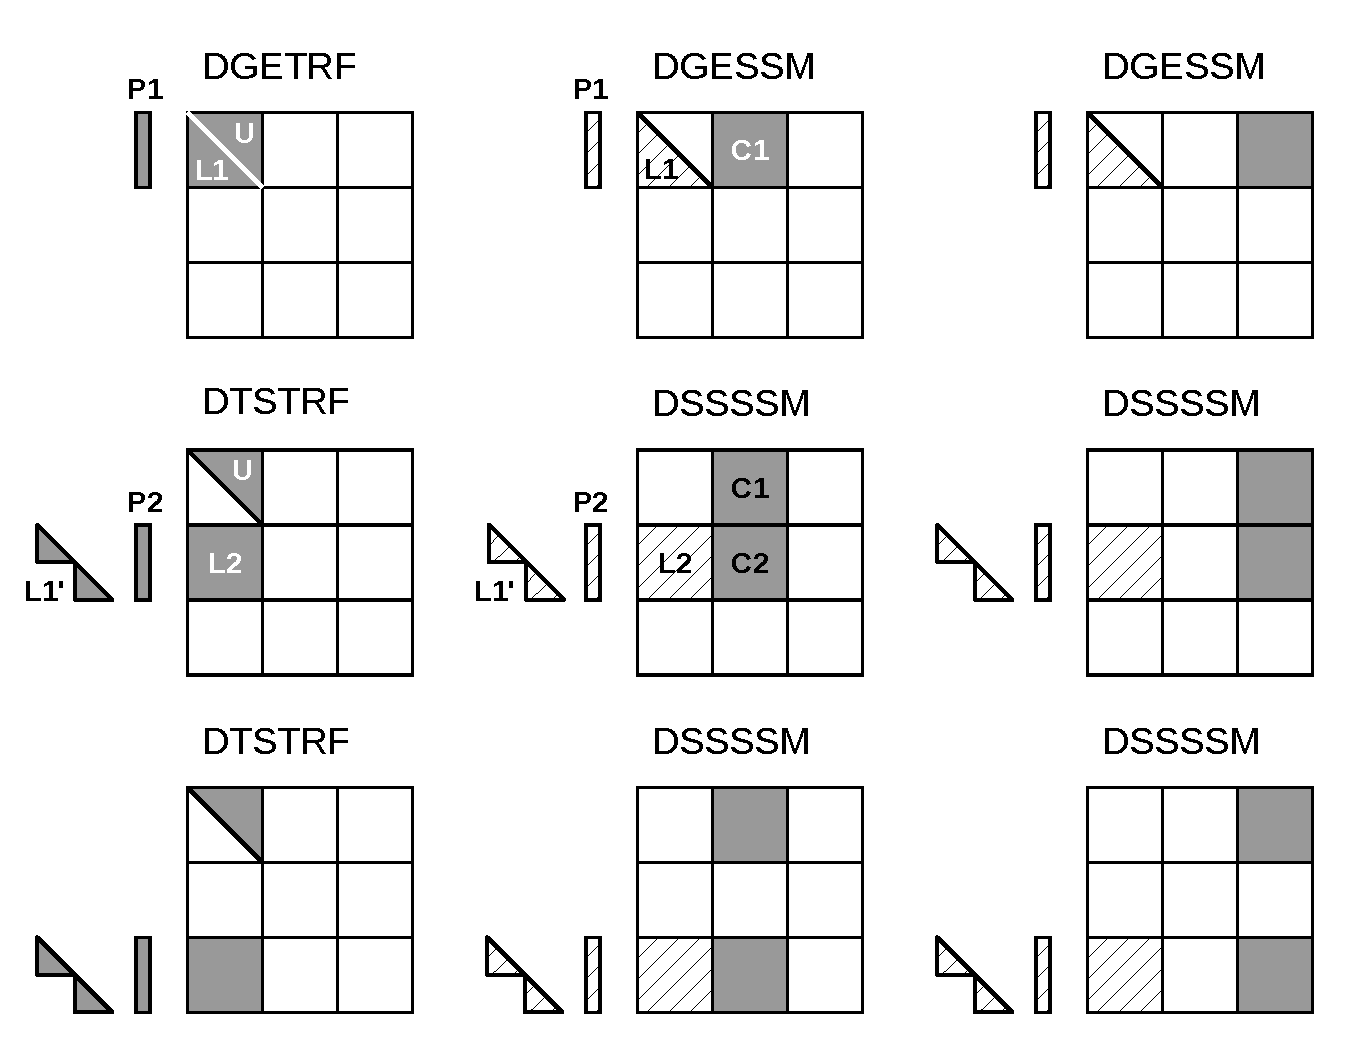
\includegraphics[width=0.60\columnwidth]{figures/tile_lu.pdf}
\caption{Schematic illustration of the tile LU factorization
         (kernel names for real arithmetics in double precision).}
\label{fig:tile_lu}
\end{figure}

%//////////////////////////////////////////////////////////

\subsection{Tile Data Layout}

Tile layout is based on the idea of storing the matrix by square tiles of relatively
small size, such that each tile occupies a continuous memory region.
This way a tile can be loaded to the cache memory efficiently and the risk of evicting it
from the cache memory before it is completely processed is minimized.
Of the three types of cache misses, {\em compulsory}, {\em capacity} and {\em conflict},
the use of tile layout minimizes the number of conflict misses, since a continuous region
of memory will completely fill out a \mbox{set-associative} cache memory before an eviction
can happen.
Also, from the standpoint of multithreaded execution, the probability of {\em false sharing}
is minimized. It can only affect the cache lines containing the beginning and the ending of a tile.

In standard \mbox{cache-based} architecture, tiles continously laid out in memory maximize
the profit from automatic prefetching.
Tile layout is also beneficial in situations involving the use of accelerators, where explicit
communication of tiles through DMA transfers is required, such as
moving tiles between the system memory and the local store in Cell B.~E. or moving tiles between
the host memory and the device memory in GPUs.
In most circumstances tile layout also minimizes the number of TLB misses and conflicts to memory
banks or partitions.
With the standard (\mbox{column-major}) layout, access to each column of a tile is much more likely
to cause a conflict miss, a false sharing miss, a TLB miss or a bank or partition conflict.
The use of the standard layout for dense matrix operations is a performance minefield.
Although occasionally one can pass through it unscathed, the risk of hitting a spot deadly to
performance is very high.

Another property of the layout utilized in PLASMA is that it is ``flat'', meaning that it does
not involve a level of indirection. Each tile stores a small square submatrix of the main matrix
in a \mbox{column-major} layout. In turn, the main matrix is an arrangement of tiles immediately
following one another in a \mbox{column-major} layout.
The offset of each tile can be calculated through address arithmetics and does not involve pointer
indirection.
Alternatively, a matrix could be represented as an array of pointers to tiles, located anywhere
in memory. Such layout would be a radical and unjustifiable departure from LAPACK and ScaLAPACK.
Flat tile layout is a natural progression from LAPACK's \mbox{column-major} layout and ScaLAPACK's
\mbox{block-cyclic} layout.

Another related property of PLASMA's tile layout is that it includes provisions for padding of tiles,
i.e., the actual region of memory designated for a tile can be larger than the memory occupied by
the actual data.
This allows to force a certain alignment of tile boundaries, while using the flat organization
described in the previous paragraph.
The motivation is that, at the price of small memory overhead, alignment of tile boundaries may
prove benefivial in multiple scenarios involving memory systems of standard multicore processors,
as well as accelerators.
The issues that come into play are, again, the use of TLBs and memory banks or partitions.

\begin{SCfigure}
\centering
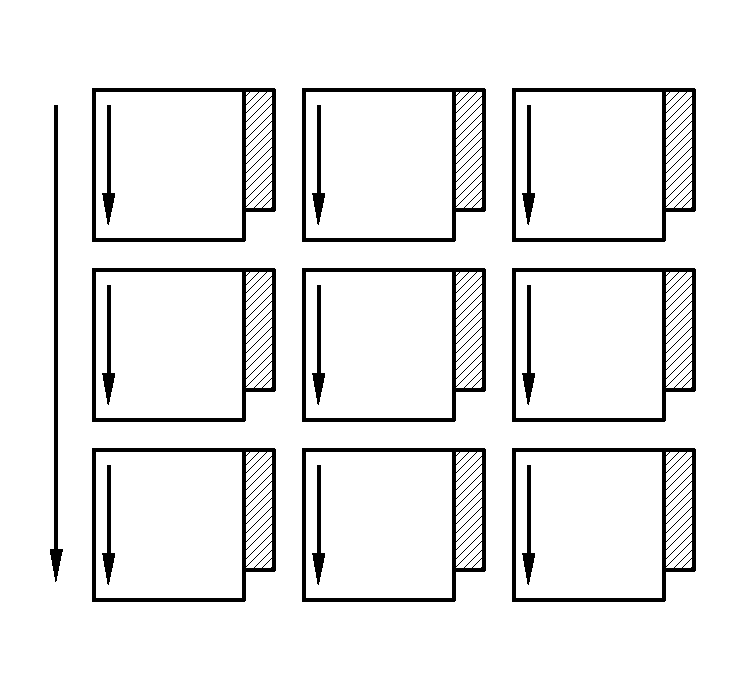
\includegraphics[width=0.5\columnwidth]{figures/tile_layout.pdf}
\caption{Schematic illustration of the tile layout with \mbox{column-major}
         order of tiles, \mbox{column-major} order of elements within tiles
         and (optional) padding for enforcing a certain alighment of tile bondaries.}
\label{fig:tile_layout}
\end{SCfigure}

%//////////////////////////////////////////////////////////

\subsection{Dynamic Task Scheduling}

Dynamic scheduling is the idea of assigning work to cores based on the availability of data
for processing at any given point in time and is also referred to as \mbox{\em data-driven}
scheduling.
The concept is related closely to the idea of expressing computation through a task graph,
often referred to as the DAG ({\em Direct Acyclic Graph}), and the flexibility exploring
the DAG at runtime.
Thus, to a large extent, dynamic scheduling is synonymous with \mbox{\em runtime scheduling}.
An important concept here is the one of the {\em critical path}, which defines the upper bound
on the achievable parallelism, and needs to be pursued at the maximum speed.
This is in direct opposition to the \mbox{\em fork-and-join} or \mbox{\em data-parallel}
programming models, where artificial synchronization points expose serial sections of
the code, where multiple cores are idle, while sequential processing takes place.
The use of dynamic scheduling introduces a \mbox{trade-off}, though.
The more dynamic (flexible) scheduling is, the more centralized (and less scalable)
the scheduling mechanism is.
For that reason, currently PLASMA uses two scheduling mechanisms, one which is fully dynamic
and one where work is assigned statically and dependency checks are done at runtime.

The first scheduling mechanism relies on unfolding a {\em sliding window} of the task graph
at runtime and scheduling work by resolving data hazards: {\em Read After Write~(RAW)},
{\em Write After Read~(WAR)} and {\em Write After Write~(WAW)}, a techniqe analogous
to instruction scheduling in superscalar processors.
It also relies on \mbox{\em work-stealing} for balanding the load among all multiple cores.
The second scheduling mechanism relies on statically designating a path through the execution
space of the algorithm to each core and following a cycle: transition to a task, wait for its
dependencies, execute it, update the overall progress.
Task are identified by tuples and task transitions are done through locally evaluated formulas.
Progress information can be centralized, replicated or distributed (currently centralized).

\begin{figure}[h!]
\centering
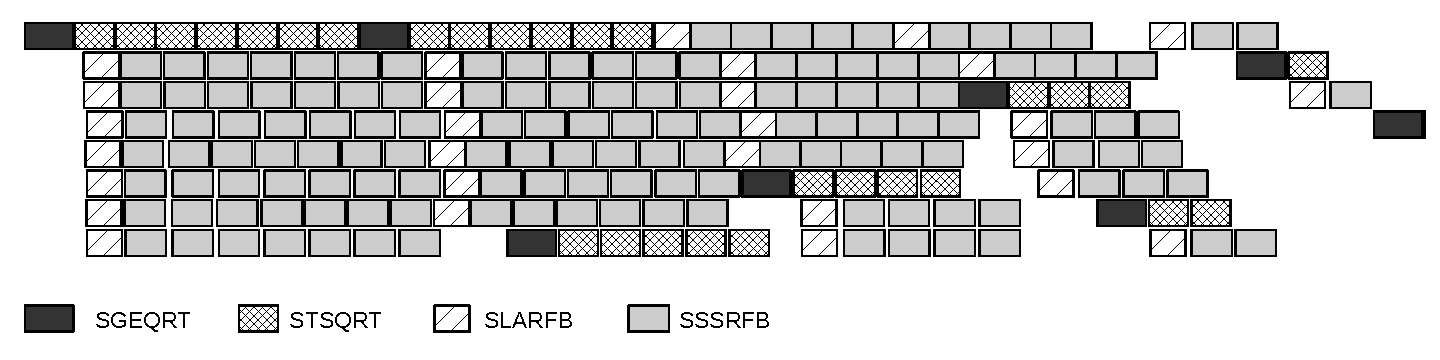
\includegraphics[width=0.8\columnwidth]{figures/trace_qr.pdf}
\caption{A trace of the tile QR factorization executing on eight cores
         without any global synchronization points
         (kernel names for real arithmetics in single precision).}
\label{fig:cholesky_trace}
\end{figure}

%//////////////////////////////////////////////////////////////////////////////////////////////////

\section{Software Stack}

Starting from the PLASMA Version 2.2, release in July 2010, the library is built on top of standard
software components, all of which are either available as open source or are standard OS facilities.
Some of them can be replaced by packages provided by hardware vendors for efficiency reasons.
Figure~\ref{fig:software_stack} presents the current structure of PLASMA's software stack.
Following is the \mbox{bottom-up} description of individual components.

\begin{figure}[h!]
\centering
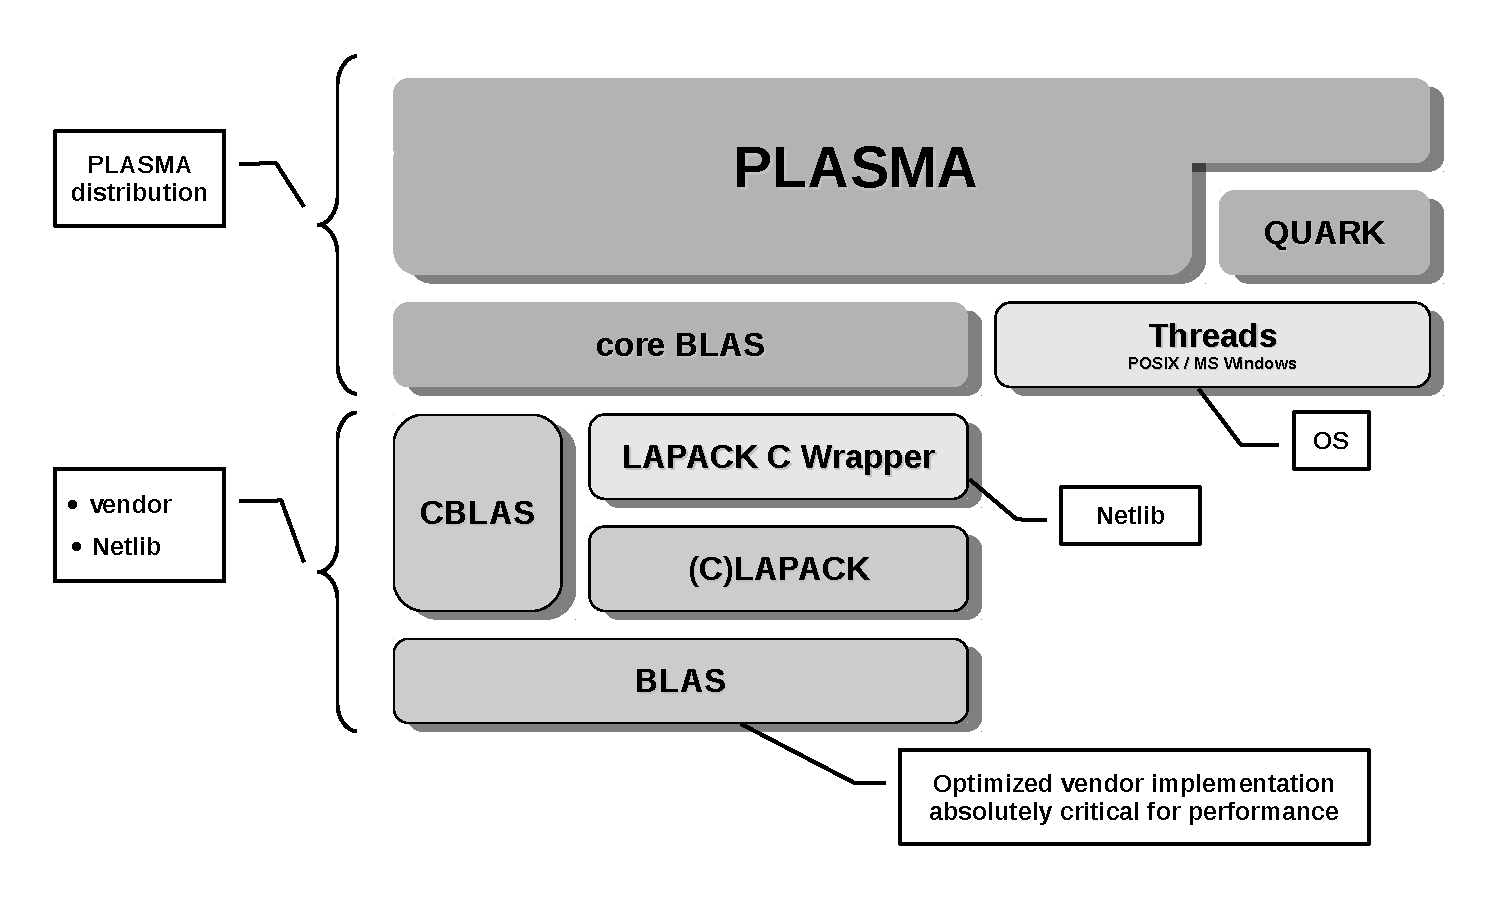
\includegraphics[width=0.8\columnwidth]{figures/software_stack.pdf}
\caption{The software stack of PLASMA Version 2.3.}
\label{fig:software_stack}
\end{figure}

\begin{description}
\item[BLAS]
is a set of Basic Linear Algebra Subprograms, a {\em de facto} standard for basic linear algebra
operations such as vector and matrix multiplication.
The definition of BLAS is available from Netlib in the form of unoptimized FORTRAN code.
Highly optimized implementations are available from many hardware vendors, such as Intel and AMD.
Fast implementations are also available in the form of academic packages, such as Goto BLAS
and ATLAS.
The standard interface to BLAS is the FORTRAN interface.

\item[CBLAS]
is the C language interface to BLAS.
The definition of CBLAS is available from Netlib in the form of a set of C wrappers for BLAS
with FORTRAN interface. Most commercial and academic implementations of BLAS also provide CBLAS.
Most people refer to CBLAS as a thin C language interoperability layer on top of an actual
implementation available through a FORTRAN interface.

\item[LAPACK]
(Linear Algebra PACKage) is a software library for numerical linear algebra, a direct predecessor
of PLASMA, providing routines for solving linear systems of equations, linear least square problems,
eigenvalue problems and singular value problems.
Many commercial and academic implementations of BLAS include a small subset of most common LAPACK
routines, such as LU, Cholesky and QR factorizations.
PLASMA uses a subset of LAPACK routines commonly provided with BLAS.

CLAPACK is a version of LAPACK available from Netlib created by automatically translating FORTRAN
LAPACK to C with the help of the F2C utility.
It provides LAPACK functionality in situations when only a C compiler is available.
At the same time, it provides the same calling convention as the ``original'' LAPACK,
the FORTRAN interface that conforms, for the most part, to the GNU g77 Application Binary
Interface~(ABI).

\item[LAPACK C Wrapper]
is a C language interface to LAPACK (or CLAPACK).
While at the time of writting this guide the effort is underway to standardize the C interface
to LAPACK, it has not been finalized yet.
For the time being, an implementation of the C interface is provided by Netlib.
Since it has not been standardized yet, it is not available from any other source.

\item[core BLAS]
is a set of serial kernels, the building blocks for PLASMA algorithms.
Ideally, core BLAS would be imlemented as monolythic kernels that are carefully optimized
for a given architecture.
This amounts, however, to a prohibitive coding effort mainly due the challenges of SIMD'zation
for vector extensions ubiquitous in modern processors.
Instead, these kernels are currently constructed from calls to BLAS and LAPACK, which is a suboptimal
way of implementing them, but the only feasible one known to the authors.

\item[Threads]
are the main mechanism for parallelization in PLASMA.
Currently relies on basic threading facilities such as launching and merging of threads,
mutexes and conditional variables.
Currently PLASMA natively supports POSIX threads and Microsoft Windows threads.

\item[QUARK]
is a simple dynamic scheduler provided with the PLASMA distribution, similar in desing principles
to the Jade project from the Massachusetts Institute of Technology, the SMPSs system from the
Barcelona Supercomputer Center, and the StarPU system from INRIA Bordeaux.
While sharing multiple slimilarities with the other projects, QUARK provides a number of extensions
necessary for integration with a numerical library such as PLASMA.
Besides serving as a component of PLASMA, QUARK is a \mbox{stand-alone} scheduler and can be
easily used outside of PLASMA.

\end{description}

One can observe that while
CBLAS provides the C interface to BLAS without the actual implementation,
CLAPACK provides the implementation of LAPACK without the actual C interface.

%//////////////////////////////////////////////////////////////////////////////////////////////////




%##################################################################################################

%%##################################################################################################

\chapter{Contents of PLASMA}

%###################################################################################################

PLASMA provides routines to solve dense general systems of linear equations,
symmetric positive definite systems of linear equations and linear least squares
problems, using LU, Cholesky, QR and LQ factorizations. Real arithmetic and complex
arithmetic are supported in both single precision and double precision.

PLASMA has been designed to supercede LAPACK and ScaLAPACK, principally by
restructuring the software to achieve much greater efficiency, where possible,
on modern computers based on multicore processors. PLASMA also relies on new or
improved algorithms. Currently, however, PLASMA does not serve as a complete
replacement of LAPACK due to limited functionality. Specifically, PLASMA does
not support band matrices and does not solve eigenvalue and singular value
problems. Also, PLASMA does not replace ScaLAPACK as software for distributed
memory computers, since it only supports shared-memory machines.


%##################################################################################################

\chapter{Installing PLASMA\label{install}}

%###################################################################################################

The requirements for installing PLASMA on a UNIX\textsuperscript{TM} system are
a C compiler, a Fortran compiler and several external libraries:
\begin{itemize}
\item a BLAS library
\item a CBLAS library
\item a LAPACK library
\item a Matrix generation library (TMG from LAPACK)
\item a C wrapper for LAPACK library
\item and the availability of the \textsf{pthread}
library.
\item The HWLoc library is also strongly recommended but not absolutely required. (\url{http://www.open-mpi.org/projects/hwloc/})
\end{itemize}
Several BLAS libraries include directly a part of this
requirements. You can refer to the table \ref{tab:extlibs} to see what
is provided by your BLAS library. 
For requirement and instructions on Microsoft Windows\textsuperscript{TM}
see Section~\ref{sec:wininstall}.
Before PLASMA can be built or tested, you must define all machine-specific parameters
for the architecture on which you are installing PLASMA.
All machine-specific parameters are contained in the file
\texttt{make.inc}. Some examples are provided in the \texttt{makes}
directory. 
To ease the installation process, we provide an installer which can
download the missing libraries from NetLib, install them and generate
the required machine-specific \texttt{make.inc} file. Users 
are strongly encouraged to use it.

\begin{table}[!htb]
  \centering
  \caption{External libraries provided by BLAS}
  \label{tab:extlibs}  
  
  \begin{tabular}{| l | c | c | c | c | c |}
    \hline
    \bf{BLAS Library}& \bf{BLAS} & \bf{CBLAS} & \bf{LAPACK}   & \bf{TMG} & \bf{LAPACK C Wrapper} \\
    \hline
    AMD ACML         &    X      &     -      &       X       &     -    &       -               \\
    \hline
    ATLAS            &    X      &     X      &       -       &     -    &       -               \\
    \hline
    GotoBLAS         &    X      &     -      &       -       &     -    &       -               \\
    \hline
    GotoBLAS2        &    X      &     X\footnote{Depends on your Makefile.rule}      &       X       &     -    &       -   \\
    \hline
    IBM ESSL         &    X      &     -      &    With CCI\footnote{\url{http://www.netlib.org/lapack/essl/}} &     -    &       -               \\
    \hline
    Intel MKL        &    X      &     X      &       X       &     X    &       -               \\
    \hline                                                                       
    refblas          &    X      &     X      &       -       &     -    &       -               \\
    \hline
    Veclib (Mac OS/X)&    \multicolumn{5}{c|}{Veclib is actually not supported}                  \\
    \hline
  \end{tabular}

\end{table}


\section{Getting the PLASMA Installer}

The PLASMA installer is a set of python scripts developed to ease
the installation of the PLASMA library and of its requirements. It can
automatically download, configure and compile the PLASMA library
including the libraries required by PLASMA.

It is available on PLASMA download page:
\begin{link_url}
\url{http://icl.cs.utk.edu/plasma/software/}
\end{link_url}

\section{PLASMA Installer Flags}

Here's a list of the flags that can be used to provide the installer
with information about the system, for example, the C and Fortran
compilers, the location of a local BLAS library, or whether the
reference BLAS needs to be downloaded.

\begin{verbatim}
./setup.py

   -h or --help
          display this help and exit

   --prefix=[DIR] 
          install files in DIR [./install]

   --build=[DIR] 
          libraries are built in DIR [./build]
          Contains log, downloads and builds.

   --cc=[CMD] 
          the C compiler. [cc]

   --fc=[CMD] 
          the Fortran compiler. [gfortran]

   --cflags=[FLAGS] 
          the flags for the C compiler [-02]

   --fflags=[FLAGS] 
          the flags for the Fortran compiler [-O2]

   --ldflags_c=[flags] 
          loader flags when main program is in C. Some
          compilers (e.g. PGI) require different
          options when linking C main programs to
          Fortran subroutines and vice-versa

   --ldflags_fc=[flags] 
          loader flags when main program is in
          Fortran. Some compilers (e.g. PGI) require
          different options when linking Fortran main
          programs to C subroutines and vice-versa.
          If not set, ldflags_fc = ldflags_c.

   --make=[CMD] 
          the make command [make]

   --blaslib=[LIB] 
          a BLAS library

   --cblaslib=[LIB] 
          a CBLAS library

   --lapacklib=[LIB] 
          a Lapack library

   --lapclib=[DIR] 
          path to a LAPACK C wrapper.

   --downblas 
          Download and install reference BLAS.

   --downcblas 
          Download and install reference CBLAS.

   --downlapack 
          Download and install reference LAPACK.

   --downlapc 
          Download and install reference LAPACK C Wrapper.

   --downall 
          Download and install all missing external libraries.
           If you don't have access to wget or no network
          connection, you can provide the following packages
          in the directory builddir/download:
     http://netlib.org/blas/blas.tgz
     http://www.netlib.org/blas/blast-forum/cblas.tgz
     http://www.netlib.org/lapack/lapack.tgz
     http://icl.cs.utk.edu/projectsfiles/plasma/pubs/lapack_cwrapper.tgz
     http://icl.cs.utk.edu/projectsfiles/plasma/pubs/plasma.tar.gz

   --[no]testing 
          enables/disables the testings. All externals
          libraries are required and tested if enabled.
          Enable by default.

   --nbcores 
          The number of cores to be used by the testing. [2]

   --clean 
          cleans up the installer directory.
\end{verbatim}

The installer will set the following environment variables 
\begin{verbatim}
	OMP_NUM_THREADS=1
	GOTO_NUM_THREADS=1
	MKL_NUM_THREADS=1
\end{verbatim}
in order to disable multithreading within BLAS. \textbf{IMPORTANT} Do
not forget to set those environment variables for any further usage of
the PLASMA libraries.  

\section{PLASMA Installer Usage}

For an installation with {\bf gcc, gfortran and reference BLAS}
\begin{verbatim}
./setup.py --cc gcc --fc gfortran --downblas
\end{verbatim}

For an installation with {\bf ifort, icc and MKL} (em64t architecture)
\begin{verbatim}
./setup.py --cc icc --fc ifort --blaslib="-lmkl_em64t -lguide"
\end{verbatim}

%% For an installation with {\bf gcc, gfortran and Veclib} (Mac OS/X)
%% \begin{verbatim}
%% ./setup.py --cc gcc --fc gfortran --blaslib="-framework veclib"
%% \end{verbatim}

For an installation with {\bf gcc, gfortran, ATLAS}
\begin{verbatim}
./setup.py --cc gcc --fc gfortran --blaslib="-lf77blas -lcblas -latlas"
\end{verbatim}

For an installation with {\bf gcc, gfortran, goto BLAS and 4 cores}
\begin{verbatim}
./setup.py --cc gcc --fc gfortran --blaslib="-lgoto" --nbcores=4
\end{verbatim}

For an installation with {\bf xlc, xlf, essl and 8 cores}
\begin{verbatim}
./setup.py --cc xlc --fc xlf --blaslib="-lessl" --nbcores=8
\end{verbatim}


\section{PLASMA Installer Support}

Please note that this is an alpha version of the installer and, even though
it has been tested on a wide set of systems, it may not work. If you
encounter a problem, your feedback would be greatly appreciated and
would be very useful for improving the quality of this installer.
Please submit your complaints and suggestions to the PLASMA forum:
\begin{link_url}
\url{http://icl.cs.utk.edu/plasma/forum/}
\end{link_url}
              
\section{Tips and Tricks\label{tips}}

\subsection{Tests are slow}
If the installer is asked to automatically download and install a BLAS
library (using the \texttt{--downblas} flag), the reference BLAS from
Netlib is installed and very low performance is to be expected.  It is
strongly recommended that you use an optimized BLAS library (such as
ATLAS, Cray Scientific Library, HP MLIB, Intel MKL, GotoBLAS, IBM ESSL,
VecLib etc.) and provide its location
through the \texttt{--blaslib} flag.

\subsection{Installing BLAS on a Mac}
Optimized BLAS are available using \texttt{VecLib} if you install the
Xcode developer package provided with your Mac OS installation CD.  On
MAC OS/X you may be required to add the following flag.
\begin{verbatim}
--ccflags="-I/usr/include/sys/"
\end{verbatim}

\subsection{Processors with Hyper-threading}
The PLASMA installer cannot detect if you have hyper-threading enabled
on your machine, if you don’t use HWLoc library. In this case, we
advise you to limit the number of cores for the initial testing of the
PLASMA library to half the numbers of cores available if you do not
know your exact architecture.  Using hyper-threading will cause the
PLASMA testing to hang.  When using PLASMA, the number of cores should
not exceed the number of actual compute cores (ignore cores appearing
due to hyper-threading).

\subsection{Problems with Downloading}
If the required packages cannot be automatically downloaded (for
example, because no network connection is available on the
installation system),
you can obtain them from the following URLs and place
them in the build subdirectory of the installer  (if the directory does not exist, create
it):
\begin{description}
\item[BLAS] Reference BLAS written in Fortran can be obtained from
\begin{link_url}
\url{http://netlib.org/blas/blas.tgz}
\end{link_url}
\item[PLASMA] The PLASMA source code is available via a link on the download page:
\begin{link_url}
\url{http://icl.cs.utk.edu/plasma/software/}
\end{link_url}
\end{description}


\section{PLASMA under Windows}
\label{sec:wininstall}
We provide installer packages for 32-bit and 64-bit binaries on
Windows available from the PLASMA web site.  
\begin{link_url}
\url{http://icl.cs.utk.edu/plasma/software/}
\end{link_url}
These Windows packages are created using Intel C and Fortran compilers
using multi-threaded static linkage, and the packages should include
all required redistributable libraries.  The binaries included in this
distribution link the PLASMA libraries with Intel MKL BLAS in order to
provide basic functionality tests.  However, any BLAS library should
be usable with the PLASMA libraries.

\subsection{Using the Windows PLASMA binary package}
Using the PLASMA libraries requires at least a C99 or C++ compiler and a
BLAS implementation.  The \texttt{examples} directory contains several examples
of using PLASMA's linear algebra functions and a simplified makefile
(\texttt{Makefile.nmake}).  This file provides guidance on how to
compile and link C or Fortran code using several different compilers
(Microsoft Visual C, Intel C, Intel Fortran) and different BLAS
libraries (Intel MKL, AMD ACML) in 32- or 64-bit floating-point precisions.
The examples in \texttt{Makefile.nmake} will have to be adjusted to the
appropriate locations of the compilers and libraries.

You \textbf{need} to make sure that the BLAS libraries are being used
in a sequential mode, either by linking with a sequential version of the
BLAS libraries, or by setting the appropriate environment variable for
that library.  PLASMA manages the parallelism on a machine and it will
cause substantial performance degradation and a possible hang of the code
if the BLAS calls are also running in parallel.

\subsection{Building PLASMA libraries}
Rebuilding the PLASMA libraries should not be required, but if you
wish to do so, the tested build environment uses Intel C and Fortran
compilers, Intel MKL BLAS, and the CMake build system.  This build
enforces an out-of-source build to avoid clobbering pre-existing
files.  The following example commands show how the build might be
done from a command shell window where the path has been setup for the appropriate
(either 32-bit or 64-bit) Intel environment.
\begin{verbatim}
mkdir BUILD
cd BUILD
cmake -DCMAKE_Fortran_COMPILER=ifort -DCMAKE_C_COMPILER=icl 
      -DCMAKE_CXX_COMPILER=icl -G "NMake Makefiles" ..
nmake
\end{verbatim}

Native threading API (as supplied with modern Windows systems starting
with Windows 2000) is used to provide parallelism within the PLASMA code.
Wrapper functions translate any PLASMA threading calls into native Windows
thread calls.  For example, the \textsf{\_beginthreadex()} function is called
to spawn PLASMA threads.

%##################################################################################################

\chapter{PLASMA Testing Suite}

%###################################################################################################
There are two distinct sets of test programs for PLASMA routines,
simple test programs written in C and advanced test programs written
in Fortran.  These programs test the linear equation routines
(eigensystem routines are not yet available) in each data type
single, double, complex, and double complex (sdcz).

\section{Simple Test Programs}
In the \texttt{testing} directory, you will find simple C codes which
test the \texttt{PLASMA\_[sdcz]gels}, \texttt{PLASMA\_[sdcz]gesv},
\texttt{PLASMA\_[sdcz]posv} routines as well as routines using iterative refinement 
for LU factorization using random matrices.  Each solving routine is
also tested using different scenarios. For instance, testing complex
least square problems on tall matrices is done by a single call to
\texttt{PLASMA\_zgels} as well as successive calls to \texttt{PLASMA\_zgeqrf},
\texttt{PLASMA\_zunmqr} and \texttt{PLASMA\_ztrsm}.

A python script \texttt{plasma\_testing.py} runs all testing routines
in all precisions. This script can take the number of cores to run the 
testing as a parameter, the default being half of the cores available.

A brief summary is printed out on the screen as the testing procedure runs. A detailed summary is written
in \texttt{testing\_results.txt} at the end of the testing phase and
can be sent the PLASMA development group if any 
failures are encountered (see Section~\ref{sec:contact}).

Each test can also also be run individually. The usage of each test is
shown by typing the desired  
testing program without any arguments. For example:
\begin{verbatim}
> ./testing_cgesv 
 Proper Usage is : ./testing_cgesv ncores N LDA NRHS LDB with 
 - ncores : number of cores 
 - N : the size of the matrix 
 - LDA : leading dimension of the matrix A 
 - NRHS : number of RHS 
 - LDB : leading dimension of the matrix B 
\end{verbatim}

\section{Advanced Test Programs}
In the \texttt{testing/lin} directory, you will find Fortran codes which check
the \texttt{PLASMA\_[sdcz]gels}, \texttt{PLASMA\_[sdcz]gesv} and \texttt{PLASMA\_[sdcz]posv} routines. 
This allows us to check not only the correctness of the routines but also the PLASMA 
Fortran interface. This test suite has been taken from LAPACK 3.2 with
necessary modifications to safely integrate PLASMA routine calls.

There is also a python script called \texttt{lapack\_testing.py} which tests all routines
in all precisions. A brief summary is printed out on the screen as the testing procedure runs. A detailed summary is written
in \texttt{testing\_results.txt} at the end of the testing procedure and can be sent to us if any 
failures are encountered (see Section~\ref{sec:contact}).

Each test can also be run individually.  For single, double, complex,
and double complex precision tests, the calls are respectively:
\begin{verbatim}
xlintsts < stest.in > stest.out
xlintstd < dtest.in > dtest.out
xlintstc < ctest.in > ctest.out
xlintstz < ztest.in > ztest.out
\end{verbatim}

For more information
on the test programs and how to modify the input files, please refer to LAPACK Working
Note 41~\cite{Blackford:1992:IGL}.

\section{Send the Results to Tennessee}
\label{sec:contact}
You made it! You have now finished installing and testing PLASMA. If
you encountered failures in any phase of the installing or testing
 process, please consult Chapter~\ref{sec:trouble} as well as the \texttt{README} 
file located in the root directory of your PLASMA installation.
If the suggestions do not fix your problem, please feel free to send a post 
in the PLASMA users' forum \url{http://icl.cs.utk.edu/plasma/forum/}.

Tell us the type of machine on which the tests were run, the version of the operating
system, the compiler and compiler options that were used, and details of the BLAS library
or libraries that you used. You should also include a copy of the output file in which the
failure occurs.
We encourage you to make the PLASMA library available to your users and provide us
with feedback from their experiences.

%##################################################################################################

\chapter{Use of PLASMA and Examples}

%###################################################################################################
\section{Examples}
In the \texttt{./examples} directory, you will find simple example codes to call
the PLASMA\_[sdcz]gels, PLASMA\_[sdcz]gesv and PLASMA\_[sdcz]posv routines from
a C program or from a Fortran program.  In this section we further explain the necessary
steps for a correct use of these PLASMA routines.

\section{\texttt{PLASMA\_dgesv} example}

Before calling the PLASMA routine \texttt{PLASMA\_dgesv}, some initialization steps 
are required.

Firstly, we set the dimension of the problem $Ax=B$.  In our example, the
coefficient matrix $A$ is 10-by-10, and the right-hand side matrix $B$ 10-by-5.
We also allocate the memory space required for these two matrices.
\begin{verbatim}
in C:
   int N = 10;
   int NRHS = 5;
   int NxN = N*N;
   int NxNRHS = N*NRHS;
   double *A = (double *)malloc(NxN*sizeof(double));
   double *B = (double *)malloc(NxNRHS*sizeof(double));
in Fortran:
      INTEGER           N, NRHS
      PARAMETER         ( N = 10 )
      PARAMETER         ( NRHS = 5 )
      DOUBLE PRECISION  A( N, N ), B( N, NRHS )
\end{verbatim}

Secondly, we initialize the matrix $A$ and $B$ with random values.  Since we
cruelly lack imagination, we use the LAPACK function \texttt{dlarnv} for this
task.  For a starter, you are welcome to change the values in the matrix.
Remember that the interface of \texttt{PLASMA\_dgesv} uses column major format.
\begin{verbatim}
in C:
   int IONE=1;
   int ISEED[4] = {0,0,0,1};   /* initial seed for dlarnv() */
   /* Initialize A */
   dlarnv(&IONE, ISEED, &NxN, A);
   /* Initialize B */
   dlarnv(&IONE, ISEED, &NxNRHS, B);
in Fortran:
      INTEGER           I
      INTEGER           ISEED( 4 )
      EXTERNAL          DLARNV
      DO  I = 1, 4
          ISEED( I ) = 1
      ENDDO
!--   Initialization of the matrix
      CALL DLARNV( 1, ISEED, N*N, A )

!--   Initialization of the RHS
      CALL DLARNV( 1, ISEED, N*NRHS, B )
\end{verbatim}

Thirdly, we initialize PLASMA by calling the \texttt{PLASMA\_Init} routine.
The variable \texttt{cores} specifies the number of cores PLASMA will use.
\begin{verbatim}
in C:
   int cores = 2;
    /* Plasma Initialize */
   INFO = PLASMA_Init(cores);
in Fortran:
      INTEGER     CORES
      PARAMETER   ( CORES = 2 )
      INTEGER     INFO
      EXTERNAL    PLASMA_INIT
! --  Initialize Plasma
      CALL PLASMA_INIT( CORES, INFO )
\end{verbatim}

Before we can call \texttt{PLASMA\_dgesv}, we need to allocate some workspace
necessary for the \texttt{PLASMA\_dgesv} routine to operate.
In PLASMA, each routine has its own routine to allocate its specific workspace arrays. Those
routines are all defined in the \texttt{workspace.c} file. Their names are of
the kind \texttt{PLASMA\_Alloc\_Workspace\_} with the name of the associated
routine in lower case for C and \texttt{PLASMA\_ALLOC\_WORKSPACE\_} with the
name of the associated routine in upper case for Fortran. You will also need to
check the interface since they are different from one routine to the other.
For the \texttt{PLASMA\_dgesv} routine, two arrays need to be initialized,
the workspace (here it is called \texttt{L} in the C code and \texttt{HL} in
the Fortran Code) and the pivots (here it is called \texttt{IPIV} in the C code
and \texttt{HIPIV} in the Fortran Code). Note that in C, you need to use
standard pointers; while in Fortran, you need to use handle defined as an array
of two elements of \texttt{INTEGER*4}.
\begin{verbatim}
in C:
   double *L;
   int *IPIV;
   PLASMA_Alloc_Workspace_dgesv(N, &L, &IPIV);
in Fortran:
      INTEGER*4         HL( 2 ), HPIV( 2 )
      EXTERNAL          PLASMA_ALLOC_WORKSPACE_DGESV
! --  Allocate L and IPIV
      CALL PLASMA_ALLOC_WORKSPACE_DGESV( N, HL, HPIV, INFO )
\end{verbatim}

Finally, 
 we can call the
\texttt{PLASMA\_dgesv} routine. You can report to
the header of the routine for a complete description of the arguments. The
description is also available online in the PLASMA routine description html
page:
\texttt{\url{http://icl.cs.utk.edu/projectsfiles/plasma/html/routine.html}}. As
in LAPACK, PLASMA is returning a return variable, \texttt{INFO}, that indicates if the
exit was successful or not. A successful exit is indicated by \texttt{INFO} equal to \texttt{0}.
In a case of \texttt{INFO} different from \texttt{0}, the value of
\texttt{INFO} should help you to understand the reason of the failure. (See the return
value section in the above cited documentation.)
\begin{verbatim}
in C:
   /* Solve the problem */
   INFO = PLASMA_dgesv(N, NRHS, A, N, L, IPIV, B, N);
   if (INFO < 0)
       printf("-- Error in DGESV example ! \n");
   else
       printf("-- Run successful ! \n");
in Fortran:
! --  Perform the LU solve
      CALL PLASMA_DGESV( N, NRHS, A, N, HL, HPIV, B, N, INFO )
      IF ( INFO < 0 ) THEN
          WRITE(*,*) " -- Error in DGESV example !"
      ELSE
          WRITE(*,*) " -- Run successful !"
      ENDIF

\end{verbatim}

Before exiting the program, we need to free the resource used by
our arrays and finalize PLASMA.
To deallocate the C array, a simple call to \texttt{free} is needed 
whereas in Fortran, PLASMA provides the 
routine \texttt{PLASMA\_DEALLOC\_HANDLE} to do so.
\texttt{PLASMA\_Finalize} call will free all the internal allocated variables and finalize PLASMA.
\begin{verbatim}
in C:
   /* Deallocate L and IPIV */
   free(L); free(IPIV);
   /* Plasma Finalize */
   INFO = PLASMA_Finalize();
in Fortran:
! --  Deallocate L and IPIV
      CALL PLASMA_DEALLOC_HANDLE( HL, INFO )
      CALL PLASMA_DEALLOC_HANDLE( HPIV, INFO )
!--   Finalize Plasma
      CALL PLASMA_FINALIZE( INFO )
\end{verbatim}




%##################################################################################################

\chapter{Performance of PLASMA}

\section{A Library for Multicore Architectures}

To achieve high performance on multicore architectures, \PLASMA
relies on tile algorithms, which provide fine granularity
parallelism. The standard linear algebra algorithms can then be
represented as Directed Acyclic Graphs (DAG) where nodes represent
tasks and edges represent dependencies among them.  Our programming
model enforces asynchronous, out of order scheduling of
operations. This concept is used as the basis for a scalable yet
highly efficient software framework for computational linear algebra
applications.

In \LAPACK, parallelism is obtained though the use of multithreaded
{\em Basic Linear Algebra Subprograms}~(\BLAS). In \PLASMA, parallelism is
no longer hidden inside the BLAS but is brought to the fore to yield
much better performance.

PLASMA performance strongly depends on tunable execution parameters
trading off utilization of different system resources.  The outer
block size (NB) trades off parallelization granularity and scheduling
flexibility with single core utilization, while the inner block size
(IB) trades off memory load with extra-flops.

\PLASMA is currently scheduled statically with a trade off between load
balancing and data reuse.

\section{Comparison to other libraries}
\label{sec:comparison}


We present here the performance of the three following one sided
factorizations: Cholesky, QR, and LU. We compare \PLASMA against
the two established linear algebra packages \LAPACK and \SCALAPACK. The
experiments were conducted on two different multicore architectures
based on Intel Xeon EMT64 and IBM Power6.

\PLASMA, \LAPACK and \SCALAPACK are all linked with the optimized
vendor \BLAS available on the system provided within Intel \MKL 10.1
and IBM \ESSL 4.3 on the \Intel and \Power architectures,
respectively. The first architecture is a quad-socket quad-core
machine based on an Intel Xeon EMT64 E7340 processor operating at
$2.39$ GHz. Its theoretical peak is equal to $9.6$ Gflop/s/ per core
or $153.2$ Gflop/s for the whole node (16 cores). The second
architecture is a SMP node composed of 16 dual-core Power6
processors. Each dual-core Power6 processor runs at $4.7$ GHz, leading
to a theoretical peak of $18.8$ Gflop/s per core and $601.6$ Gflop/s
per node (32 cores).

%\section{Methodology}
%\label{sec:comparison-methodology}

We only report double precision performance numbers for simplicity purposes.
\PLASMA is tuned
with the pruned search method as described in \cite{Agullo:2009:CS1}. For
\SCALAPACK, we have tuned the data distribution parameters (p,q,nb) as
functions of the number of cores and the matrix size through an
exhaustive search.  For reference LAPACK, we have been using the
default block size (no tuning).

\ignore{
Furthermore, to capture the best possible behavior of each library, we
repeat the number of executions (up to 10 times) and we report the
highest performance obtained. We do not flush the caches before timing
a factorization\footnote{It is kernel usage, not problem size, that
  dictates whether one wish to flush the cache. Warm (or partially
  warm) cache executions are plausible for dense linear
  factorizations. For instance, sparse linear solvers, which rely on
  dense kernels, intend to maximize data reuse between successive
  calls to dense operations.}. However, the TLB (Translation Lookaside
Buffer) is flushed between two executions: the loop over the different
executions is performed in a script (rather than within the
executable) and calls several times the same executable.
}

\SCALAPACK and \PLASMA interfaces allow the user to provide data
distributed on the cores. In our shared-memory multicore environment,
because we do not flush the caches, these libraries have thus the
advantage to start the factorization with part of the data distributed
on the caches. This is not negligible. For instance, a
$8000\times8000$ double precision matrix can be held distributed on
the L3 caches of the 32 cores of a \Power node.

%\subsection{Experimental results}

Figures~\ref{fig:ch}, \ref{fig:qr}, \ref{fig:lu} present performance
for the Cholesky, QR and LU factorizations, respectively.

\begin{figure}[htbp]
    \subfigure[Intel Xeon - 16 cores]{
      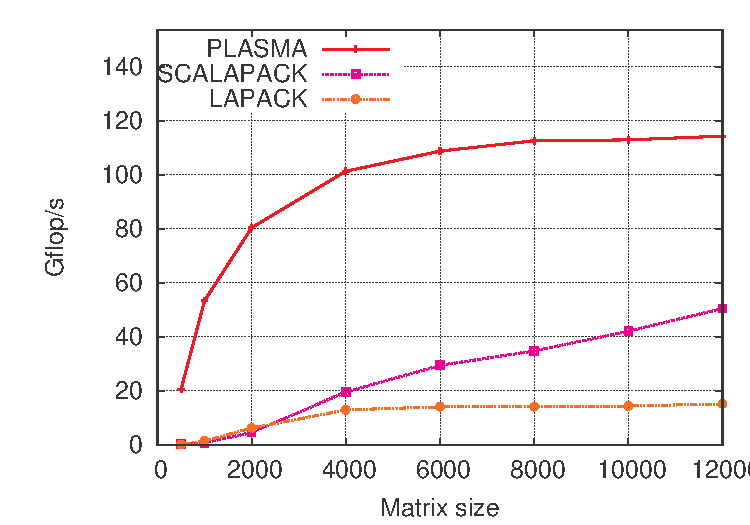
\includegraphics[width=\figwidth]{fig/Intel64-DPOTRF-PLASMA_SCALAPACK_LAPACK-16cores-short}
    }%
    \subfigure[Power6 - 32 cores]{
      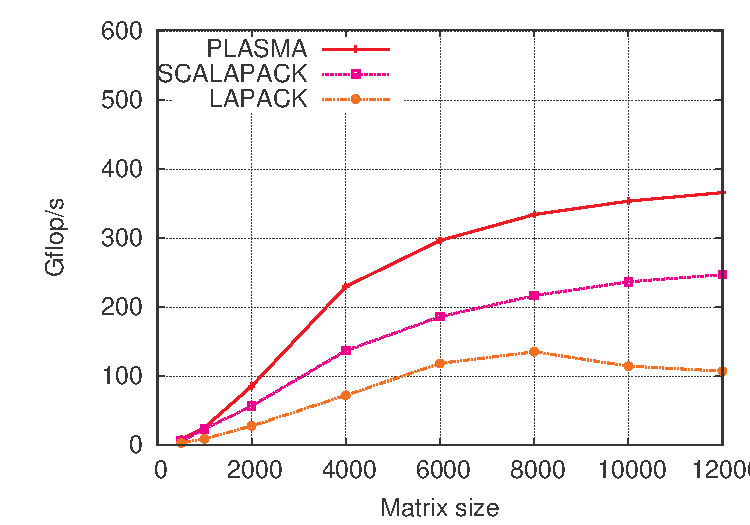
\includegraphics[width=\figwidth]{fig/Power6-DPOTRF-PLASMA_SCALAPACK_LAPACK-32cores-short}
    }%
  \caption{Performance of the Cholesky factorization (Gflop/s).}
  \label{fig:ch}
\end{figure}

\begin{figure}[htbp]
    \subfigure[Intel Xeon - 16 cores]{
      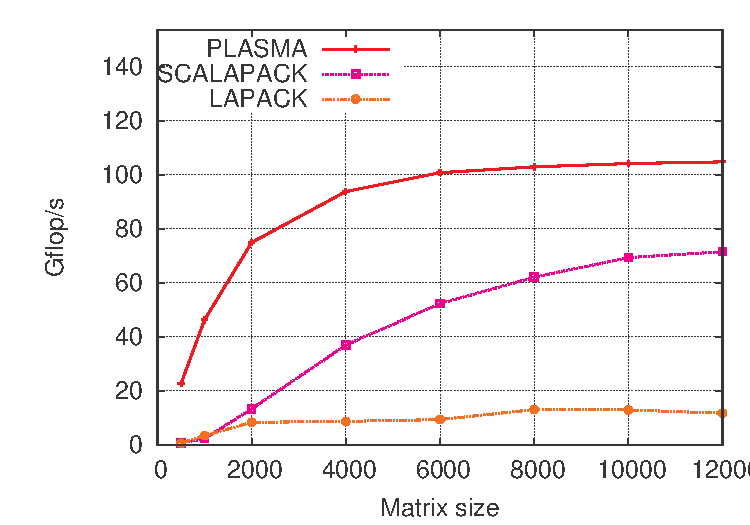
\includegraphics[width=\figwidth]{fig/Intel64-DGEQRF-PLASMA_SCALAPACK_LAPACK-16cores-short}
    }%
    \subfigure[Power6 - 32 cores]{
      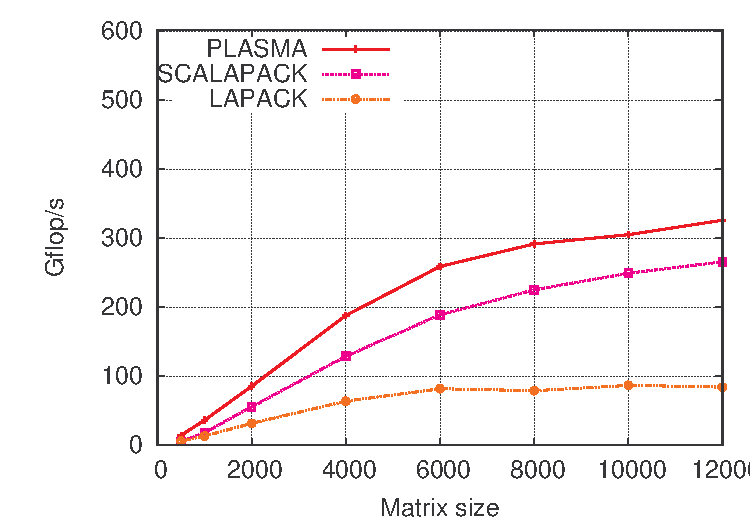
\includegraphics[width=\figwidth]{fig/Power6-DGEQRF-PLASMA_SCALAPACK_LAPACK-32cores-short}
    }%
  \caption{Performance of the QR factorization (Gflop/s).}
  \label{fig:qr}
\end{figure}

\begin{figure}[htbp]
    \subfigure[Intel Xeon - 16 cores]{
      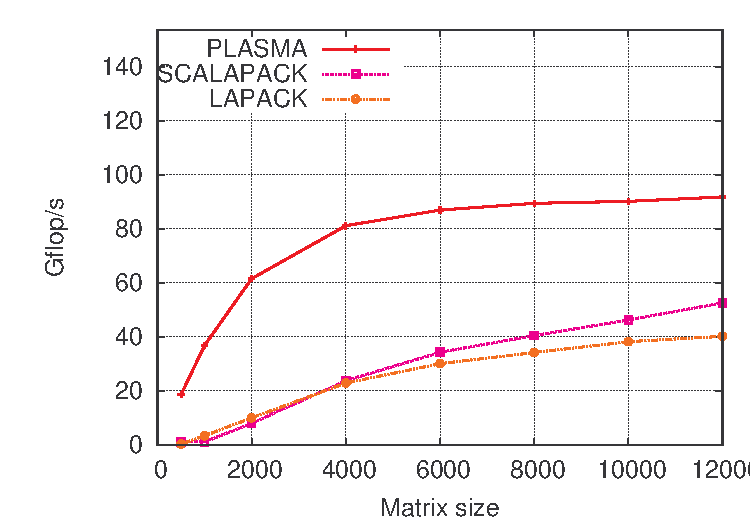
\includegraphics[width=\figwidth]{fig/Intel64-DGETRF-PLASMA_SCALAPACK_LAPACK-16cores-short}
    }%
    \subfigure[Power6 - 32 cores]{
      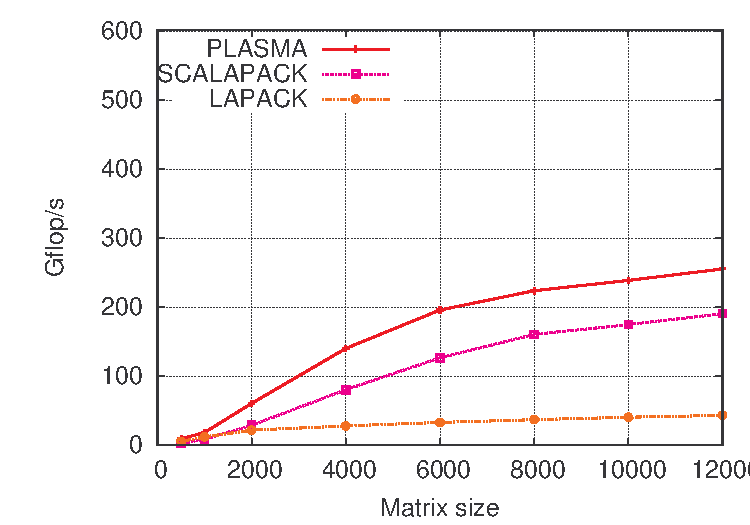
\includegraphics[width=\figwidth]{fig/Power6-DGETRF-PLASMA_SCALAPACK_LAPACK-32cores-short}
    }%
  \caption{Performance of the LU factorization (Gflop/s).}
  \label{fig:lu}
\end{figure}

\section{Tuning - Howto}

Users willing to obtain good performance from PLASMA need to tune PLASMA
parameters.  The example code below illustrates how to change the \texttt{NB}
and \texttt{IB} parameters before calling the appropriate PLASMA routine to
factorize or solve a linear system.

We recall that QR and LU algorithms requires both NB and IB parameters while Cholesky needs only NB.


\begin{verbatim}
...
       /* Plasma Tune */
       PLASMA_Disable(PLASMA_AUTOTUNING);
       PLASMA_Set(PLASMA_TILE_SIZE, NB);
       PLASMA_Set(PLASMA_INNER_BLOCK_SIZE, IB);
...
\end{verbatim}


A pruned search method to obtain ``good''
parameters is described in \cite{Agullo:2009:CS1}.  We note that autotuning is
part of the PLASMA's roadmap; unfortunately, as of 2.0.0, the PLASMA software
does not have its autotuning component available for release.

%###################################################################################################

%##################################################################################################

\chapter{Accuracy and Stability}
\newtheorem{theorem}{Theorem}[section]

%###################################################################################################


We present backward stability results of the algorithms used in PLASMA.
Backward stability is a concept developed by Wilkinson in~\cite{Wilkinson:1963:REA,Wilkinson:1965:AEP}.
For more general discussion on accuracy and stability of numerical algorithms, we refer the users to Higham~\cite{Higham:2002:ASN}.
We follow Higham's notation and methodology here; in fact, we mainly present his results.

\section{Notations}
\begin{itemize}
\item We assume the same floating-point system as Higham~\cite{Higham:2002:ASN}. His
assumptions are fulfilled by the IEEE standard. The unit round-off is $u$
which is about $1.11\times 10^{-16}$ for double.

\item The absolute value notation $|\cdot|$ is extended from scalar to matrices
where matrix $|A|$ denotes the matrix with $(i,j)$ entry $|a_{ij}|$.

\item Inequalities between matrices hold componentwise. If we write $A<B$,
this means that for any $i$ and any $j$,
$a_{ij}<b_{ij}$ ($A$ and $B$ are of the same size).

\item If $nu<1$, we define $\gamma_n \equiv \frac{nu}{1-nu}$.

\item Computed quantities are represented with an overline or with the $fl(\cdot)$ notation.

\item Inequality with $|\cdot|$ can be converted to norms easily. (See \cite[Lem.6.6]{Higham:2002:ASN}.)
\end{itemize}

\section{Peculiarity of the Error Analysis of the Tile Algorithms}

Numerical linear algebra algorithms rely at their roots on inner products.
A widely used result of error analysis of the inner product is given in Theorem~\ref{theorem:jl--1} 
\begin{theorem}\emph{(Higham, \cite[Eq.(3.5)]{Higham:2002:ASN})}
\label{theorem:jl--1}
Given $x$ and $y$, two vectors of size $n$, 
if $x^Ty$ is evaluated in floating-point arithmetic, then, 
no matter what the order of evaluation, we have
\begin{equation*}
| x^T y - fl( x^T y ) | \leq \gamma_n |x |^T |y |.
\end{equation*}
\end{theorem}
While there exists a variety of implementations and interesting research that
aim to reduce errors in inner products (see for
example~\cite[chapter~3~and~4]{Higham:2002:ASN}), we note that
Theorem~\ref{theorem:jl--1}
 is given independently of the order of evaluation in the inner
products.  The motivation for being independent of the order of evaluation is
that inner products are performed by optimized libraries which use
associativity of the addition for grouping the operations in order to obtain
parallelism and data locality in matrix-matrix multiplications.

Theorem~\ref{theorem:jl--2} presents a remark from Higham.
Higham notes that one can significantly reduce the error bound of an inner
product by accumulating it in pieces (which is indeed what an optimized BLAS library would do
to obtain performance).
\begin{theorem}\emph{(Higham, \cite[\S3.1]{Higham:2002:ASN})}
\label{theorem:jl--2}
Given $x$ and $y$, two vectors of size $n$, 
if $x^Ty$ is evaluated in floating-point arithmetic
 by accumulating the inner product in $k$ pieces of size $n/k$,
then, we have
\begin{equation*}
| x^T y - fl( x^T y ) | \leq \gamma_{n/k+k-1} |x |^T |y |.
\end{equation*}
\end{theorem}
Theorem~\ref{theorem:jl--2} has been used by
Castaldo, Whaley, and Chronopoulos~\cite{Castaldo:2008:RFP} to improve the 
error bound in matrix-matrix multiplications.

The peculiarity of tile algorithms is that they explicitly work on small pieces of data
and therefore, benefit in general from a {\em better} error bounds than their LAPACK counterparts.

\section{Tile Cholesky Factorization}

The Cholesky factorization algorithm in PLASMA performs the same operations than any version of the Cholesky.
The organization of the operations in the inner products might be different from one algorithm to the other.
The error analysis is however essentially the same for all the algorithms.

Theorem~\ref{theorem:jl--3} presents Higham's result for the Cholesky factorization.
\begin{theorem}\emph{(Higham, \cite[Th.10.3]{Higham:2002:ASN})}
\label{theorem:jl--3}
If Cholesky factorization applied to the symmetric positive definite matrix $A\in \mathbb{R}^{n\times n}$ runs to completion then the computed 
factor $\overline{R}$ satisfies 
\begin{equation*}
\overline{R}^T \overline{R} = A + \Delta A, \quad \textmd{where } | \Delta A | \leq \gamma_{n+1} |\overline{R}^T||\overline{R}|.
\end{equation*}
\end{theorem}

Following Higham's proof, we note that Higham's Equation (10.4) can be tighten in our case
since we know that the inner product are accumulated within tiles of size $b$. The $\gamma_i$ term becomes
$\gamma_{i/b+b-1}$ and we obtain the improved error bound given in
Theorem~\ref{theorem:jl--4}.
\begin{theorem}
\label{theorem:jl--4}
If {\em Tile Cholesky factorization} applied to the symmetric positive definite matrix $A\in \mathbb{R}^{n\times n}$ runs to completion then the computed 
factors $\overline{R}$ satisfies 
\begin{equation*}
\overline{R}^T \overline{R} = A + \Delta A, \quad \textmd{where } | \Delta A | \leq \gamma_{n/b+b} |\overline{R}^T||\overline{R}|.
\end{equation*}
\end{theorem}
We note that the error bound could even be made smaller by taking into account the inner blocking used in the Cholesky factorization of each tile.

Higham explains how to relate the backward error of the factorization
with the backward error of the solution of a symmetric positive definite linear system of equations.

\section{Tile Householder QR Factorization}

The {\em Tile Householder QR} is backward stable since it is obtained through a product of backward stable transformations.
One can obtain a tighter error bound with tile algorithms than with standard ones.

Higham explains how to relate the backward error of the factorization
with the backward error of the solution of a linear least squares.

\section{Tile LU Factorization}

\begin{theorem}\emph{(Bientinesi and van de Geijn, \cite[Th.6.5]{Bientinesi:2009:SDS})}
Given $A\in \mathbb{R}^{n\times n}$, assume that the blocked right-looking algorithm in Fig. 6.1 completes.
Then the computed factors $\overline{L}$ and $\overline{U}$ are such that 
\begin{equation*}
\label{theorem:jl--5}
\overline{L}\overline{U} =  A + \Delta A, \quad \textmd{where } | \Delta A | \leq \gamma_{\frac{n}{b}+b} \left( | A | + |\overline{L}||\overline{U}| \right).
\end{equation*}
\end{theorem}

We note that Bientinesi and van de Geijn do not consider permutations.

Higham explains how to relate the backward error of the factorization
with the backward error of the solution of a linear system of equations.

{\bf Words of cautions:} It is important to note that Theorem~\ref{theorem:jl--5} does not state that the algorithm is stable.
For the algorithm to be stable, we need to have
\begin{equation*}
 |\overline{L}||\overline{U}| \sim | A |.
\end{equation*}
Whether this is the case or not, this is still an ongoing research topic.
Therefore, we recommend users to manipulate \texttt{PLASMA\_dgesv} with care.
In case of doubt, it is better to use  \texttt{PLASMA\_dgels}.

%%##################################################################################################

\chapter{Documentation and Software Conventions}

%###################################################################################################

%##################################################################################################

\chapter{Troubleshooting}
\label{sec:trouble}
%##################################################################################################

\section{Wrong Results}

PLASMA is a software package distributed in source code, subject to different hardware / software
configurations.
PLASMA may deliver wrong numerical results due to a number of problems outside of PLASMA, such as:
\begin{itemize}
\item aggressive compiler optimizations violating code correctness,
\item aggressive compiler optimizations violating IEEE floating point standard,
\item hardware floating point arithmetic implementations violating IEEE standard,
\item ABI differences between compilers, if mixing compilers,
\item aggressive optimizations in BLAS implementations,
\item bugs in BLAS implementations.
\end{itemize}

PLASMA is distributed with an installer with the intention to spare the user the process
of setting up compilation and linking options.
Nevertheless, it might become necessary for the user to do so.
In such circumstances, the following recommendations should be followed.

When building PLASMA, it is recommended that dangerous compiler optimizations are avoided and
instead flags enforcing IEEE compliance are used.
It is generally recommended that ``-O2'' optimization level is used and not higher.
Users are strongly cautioned against using different compilers for PLASMA and BLAS
when building BLAS from source code.
Users are also strongly advices to pay attention to the linking sequence and follow
vendor recommendations, when vendor BLAS is used.

PLASMA software is tested daily by running a subset of LAPACK testing suite.
Each pass involves hundreds of thousands of tests including both test for numerical results,
as well as tests for detection of input errors, such as invalid input parameters.
Currently the hardware / software configurations (in different combinations) known to pass
all the tests include the following architectures:

\subsection{Linux machine: Intel x86-64}
% ZOOT TESTINGS BUILDBOT
\begin{tabular}{| c | c | c | c | c |}
\hline
C compiler & Fortran compiler & BLAS                & testing     &  testing/lin \\ 
\hline \hline
GNU gcc	4.1.2      & GNU gfortran 4.1.2    & ATLAS 3.8.1         &       PASSED      &       PASSED                  \\ \hline
GNU gcc 4.1.2      & GNU gfortran 4.1.2    & GotoBLAS 1.24       &       PASSED      & info error:        160        \\ \hline
GNU gcc 4.1.2      & GNU gfortran 4.1.2    & GotoBLAS 2          &       PASSED      & numerical failure: 1 (SPO)    \\
                   &                       &                     &       PASSED      & info error:        160        \\ \hline
GNU gcc 4.1.2      & GNU gfortran 4.1.2    & Intel MKL 11.0      &       PASSED      &       PASSED                  \\ \hline
GNU gcc 4.1.2      & GNU gfortran 4.1.2    & Reference BLAS      &       PASSED      &       PASSED                  \\ \hline
Intel icc 11.0     & Intel ifort 11.0      & ATLAS 3.8.1         &       PASSED      &       PASSED                  \\ \hline
Intel icc 11.0     & Intel ifort 11.0      & GotoBLAS 1.24       &       PASSED      & numerical failure: 87 (CPO, ZPO)   \\
                   &                       &                     &       PASSED      & illegal error:     0          \\ 
                   &                       &                     &       PASSED      & info error:        188        \\ \hline
Intel icc 11.0     & Intel ifort 11.0      & GotoBLAS 2          &       PASSED      & numerical failure: 87 (CPO, ZPO)   \\
                   &                       &                     &       PASSED      & illegal error:     0          \\ 
                   &                       &                     &       PASSED      & info error:        188        \\ \hline
Intel icc 11.0     & Intel ifort 11.0      & Intel MKL 11.0      &       PASSED      &       PASSED                  \\ \hline
Intel icc 11.0     & Intel ifort 11.0      & Reference BLAS      &       PASSED      &       PASSED                  \\ \hline
\end{tabular} 

\subsection{Linux machine: Intel 32}
\begin{tabular}{| c | c | c | c | c |}
\hline
C compiler & Fortran compiler & BLAS                 & testing     &  testing/lin \\ 
\hline \hline
% LAPTOP HATEM
GNU gcc 4.3.3  & GNU gfortran 4.3.3    & Reference BLAS        &       PASSED      &       PASSED              \\ \hline
GNU gcc 4.3.3  & GNU gfortran 4.3.3    & Intel MKL 10.1        &       PASSED      &       PASSED              \\ \hline
GNU gcc 4.3.3  & GNU gfortran 4.3.3    & ATLAS 3.8.1           &       PASSED      &       PASSED              \\ \hline
GNU gcc 4.3.3  & GNU gfortran 4.3.3    & GotoBLAS 1.24         &       PASSED      &       ERROR               \\ \hline
Intel icc 11.0 & Intel ifort 11.0      & Reference BLAS        &       PASSED      &       PASSED              \\ \hline
Intel icc 11.0 & Intel ifort 11.0      & Intel MKL 10.1        &       PASSED      &       PASSED              \\ \hline
Intel icc 11.0 & Intel ifort 11.0      & ATLAS 3.8.1           &       PASSED      &       PASSED              \\ \hline
Intel icc 11.0 & Intel ifort 11.0      & GotoBLAS 1.24         &       PASSED      &       ERROR               \\ \hline
\hline
\end{tabular} 

\subsection{Linux machine: Intel Itanium}
\begin{tabular}{| c | c | c | c | c |}
\hline
C compiler & Fortran compiler & BLAS                 & testing     &  testing/lin \\ 
\hline \hline
% ANAKA BUILDBOT
GNU gcc 4.1.2      & GNU gfortran 4.1.2    & Reference BLAS  &      PASSED       &       PASSED      \\ \hline
GNU gcc 4.1.2      & GNU gfortran 4.1.2    & GotoBLAS        &      PASSED       &       PASSED      \\ \hline
GNU gcc 4.1.2      & GNU gfortran 4.1.2    & GotoBLAS 2      &      PASSED       &       PASSED      \\ \hline
GNU gcc 4.1.2      & GNU gfortran 4.1.2    & MKL             &      PASSED       &       PASSED      \\ \hline
Intel icc 11.1     & Intel icc ifort 11.1  & MKL             &      PASSED       &       PASSED      \\ \hline
% HP03 BUILDBOT
Intel icc 11.1     & Intel icc ifort 11.1  & Reference BLAS  &      PASSED       &       PASSED      \\ \hline
\hline
\end{tabular} 

\subsection{Linux machine: AMD Opteron}
\begin{tabular}{| c | c | c | c | c |}
\hline
C compiler & Fortran compiler & BLAS                 & testing     &  testing/lin \\ 
\hline \hline
% TORC10 BUILDBOT
GNU gcc 4.1.2      & GNU gfortran 4.1.2    & Reference BLAS  &      PASSED       &       PASSED      \\ \hline
GNU gcc 4.1.2      & GNU gfortran 4.1.2    & ACML 14.3.0     &      PASSED       &       PASSED      \\ \hline
% MARVIN.CS.UH.EDU HATEM AMD Opteron Processor 846
PATHSCALE pathcc  2.5 & PATHSCALE pathf90 2.5 & INTEL MKL 10.0.1 &  PASSED       &       PASSED      \\ \hline
% medusa.tlc2.uh.edu HATEM AMD Opteron Processor 242
PORTLAND pgcc 8.0-6 & PORTLAND pgf90 8.0-6 &  Reference BLAS &  PASSED       &       PASSED      \\ \hline
\hline
\end{tabular} 

\subsection{Linux machine: IBM Power6}
\begin{tabular}{| c | c | c | c | c |}
\hline
C compiler & Fortran compiler & BLAS                 & testing     &  testing/lin \\ 
\hline \hline
% BLUEGRASS
GNU gcc 4.3.1      & GNU gfortran 4.3.2    & Reference BLAS  &      PASSED       &       PASSED      \\ \hline
GNU gcc 4.3.1      & GNU gfortran 4.3.2    & ATLAS           &      PASSED       &       PASSED      \\ \hline
GNU gcc 4.3.1      & GNU gfortran 4.3.2    & ACML            &      PASSED       &       PASSED      \\ \hline
\end{tabular} 

\subsection{Non-Linux machine}
\begin{tabular}{| c | c | c | c | c | c |}
\hline
Machine &   C compiler & Fortran compiler & BLAS                 & testing     &  testing/lin \\  
\hline \hline
% SNOW JULIE
MAC OS/X Snow Leopard & GNU gcc 4.3.0 & GNU gfortran 4.3.0 & Reference BLAS     &      PASSED       &       PASSED      \\ \hline
MAC OS/X Snow Leopard & GNU gcc 4.3.0 & GNU gfortran 4.3.0 & Veclib framework   &      PASSED       &       PASSED      \\ \hline
% VARGAS EMMANUEL
AIX 5.3          & IBM XLC 10.1  & IBM XLF 12.1       & ESSL 4.3           &      PASSED       &       PASSED      \\ \hline
\end{tabular} 


Currently the hardware / software configurations known to fail PLASMA tests are:
\begin{itemize}
\item Intel x86-64, GCC, GFORTAN, Goto BLAS,
\item Intel x86-64, GCC, GFORTAN, Goto BLAS 2,
\item Intel x86-64, ICC, IFORT, Goto BLAS,
\item Intel x86-64, ICC, IFORT, Goto BLAS 2.
\end{itemize}

%###################################################################################################


%//////////////////////////////////////////////////////////////////////////////////////////////////

\bibliographystyle{unsrt}
\bibliography{users_guide}

%##################################################################################################

\end{document}
